% FID values for run2, run6 and run7
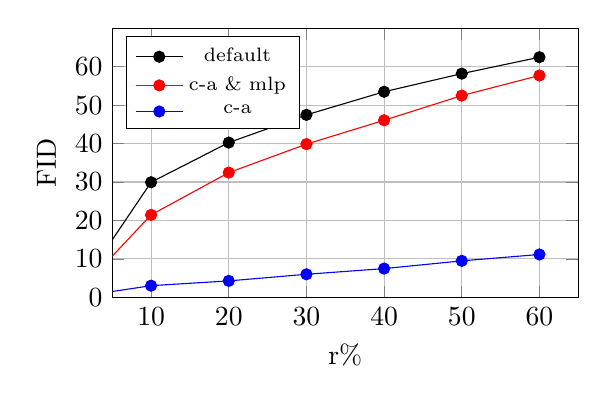
\begin{tikzpicture}
\begin{axis}[
    title={},
    height=5cm,
    width=7.5cm,
    xlabel={r\%},
    ylabel={FID},
    xmin=5, xmax=65,
    ymin=0, ymax=70,
    xtick={10,20,30,40,50,60},
    ytick={0,10,20,30,40,50,60},
    legend pos=north west,
    xmajorgrids=true,
    ymajorgrids=true,
    legend style={font=\scriptsize}
]

\addplot[
    color=black,
    mark=*
    ]
    coordinates {
    (0,0)(10,29.95)(20,40.26)(30,47.47)(40,53.48)(50,58.19)(60,62.46)
    };
    
\addplot[
    color=red,
    mark=*
    ]
    coordinates {
    (0,0)(10,21.46)(20,32.45)(30,39.86)(40,46.06)(50,52.48)(60,57.71)
    };

\addplot[
    color=blue,
    mark=*
    ]
    coordinates {
    (0,0)(10,3.05)(20,4.29)(30,6.01)(40,7.49)(50,9.50)(60,11.16)
    };

    
\legend{default, c-a \& mlp, c-a}
    
\end{axis}
\end{tikzpicture}